\begin{figure}[htbp]
  \centering
  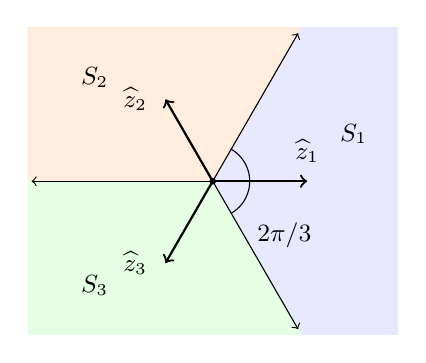
\begin{tikzpicture}[x=1cm,y=1cm,line cap=round,line join=round,
                      font=\small]
    \begin{scope}
      \clip (-2.35,-1.95) rectangle (2.35,1.95);
      \fill[blue!9] (0,0) -- (-60:8) -- (60:8) -- cycle;
      \fill[orange!13] (0,0) -- (60:8) -- (180:8) -- cycle;
      \fill[green!10!white] (0,0) -- (180:8) -- (300:8) -- cycle;
    \end{scope}
    \draw[->,thin] (0,0) -- (60:2.17);
    \draw[->,thin] (0,0) -- (180:2.30);
    \draw[->,thin] (0,0) -- (300:2.17);
    \draw[thick,->] (0,0) -- (0:1.20)
      node[above=3pt] {$\widehat z_1$};
    \draw[thick,->] (0,0) -- (120:1.20)
      node[left=3pt] {$\widehat z_2$};
    \draw[thick,->] (0,0) -- (240:1.20)
      node[left=3pt] {$\widehat z_3$};
    \draw[thin] (-60:.47) arc[start angle=-60,end angle=60,radius=.47];
    \node at (.91,-.69) {$2\pi/3$};
    \node at (1.79,.60) {$S_1$};
    \node at (-1.50,1.32) {$S_2$};
    \node at (-1.50,-1.32) {$S_3$};
    \fill (0,0) circle[radius=1.2pt];
  \end{tikzpicture}
  \caption{The attaining planar partition consists of three unbounded
  sectors $S_1,S_2,S_3$ of angle $2\pi/3$; only a finite window is shown.
  The bold arrows show the unit centroid directions
  $\widehat z_i=z(S_i)/\|z(S_i)\|$.
  Each unnormalized Gaussian centroid has length
  $\sqrt{3}/(2\sqrt{2\pi})$, so their squared lengths sum to
  $9/(8\pi)$. In dimension $d\ge2$, use
  $S_i\times\mathbb R^{d-2}$, with any further cells empty.}
  \label{fig:propeller-sectors}
\end{figure}
